\PassOptionsToPackage{unicode=true}{hyperref} % options for packages loaded elsewhere
\PassOptionsToPackage{hyphens}{url}
%
\documentclass[
  ignorenonframetext,
]{beamer}
\usepackage{pgfpages}
\setbeamertemplate{caption}[numbered]
\setbeamertemplate{caption label separator}{: }
\setbeamercolor{caption name}{fg=normal text.fg}
\beamertemplatenavigationsymbolsempty
% Prevent slide breaks in the middle of a paragraph:
\widowpenalties 1 10000
\raggedbottom
\setbeamertemplate{part page}{
  \centering
  \begin{beamercolorbox}[sep=16pt,center]{part title}
    \usebeamerfont{part title}\insertpart\par
  \end{beamercolorbox}
}
\setbeamertemplate{section page}{
  \centering
  \begin{beamercolorbox}[sep=12pt,center]{part title}
    \usebeamerfont{section title}\insertsection\par
  \end{beamercolorbox}
}
\setbeamertemplate{subsection page}{
  \centering
  \begin{beamercolorbox}[sep=8pt,center]{part title}
    \usebeamerfont{subsection title}\insertsubsection\par
  \end{beamercolorbox}
}
\AtBeginPart{
  \frame{\partpage}
}
\AtBeginSection{
  \ifbibliography
  \else
    \frame{\sectionpage}
  \fi
}
\AtBeginSubsection{
  \frame{\subsectionpage}
}
\usepackage{lmodern}
\usepackage{amssymb,amsmath}
\usepackage{ifxetex,ifluatex}
\ifnum 0\ifxetex 1\fi\ifluatex 1\fi=0 % if pdftex
  \usepackage[T1]{fontenc}
  \usepackage[utf8]{inputenc}
  \usepackage{textcomp} % provides euro and other symbols
\else % if luatex or xelatex
  \usepackage{unicode-math}
  \defaultfontfeatures{Scale=MatchLowercase}
  \defaultfontfeatures[\rmfamily]{Ligatures=TeX,Scale=1}
\fi
% use upquote if available, for straight quotes in verbatim environments
\IfFileExists{upquote.sty}{\usepackage{upquote}}{}
\IfFileExists{microtype.sty}{% use microtype if available
  \usepackage[]{microtype}
  \UseMicrotypeSet[protrusion]{basicmath} % disable protrusion for tt fonts
}{}
\makeatletter
\@ifundefined{KOMAClassName}{% if non-KOMA class
  \IfFileExists{parskip.sty}{%
    \usepackage{parskip}
  }{% else
    \setlength{\parindent}{0pt}
    \setlength{\parskip}{6pt plus 2pt minus 1pt}}
}{% if KOMA class
  \KOMAoptions{parskip=half}}
\makeatother
\usepackage{xcolor}
\IfFileExists{xurl.sty}{\usepackage{xurl}}{} % add URL line breaks if available
\IfFileExists{bookmark.sty}{\usepackage{bookmark}}{\usepackage{hyperref}}
\hypersetup{
  pdftitle={Introduction to Natural Gas},
  pdfauthor={James Woods},
  pdfborder={0 0 0},
  breaklinks=true}
\urlstyle{same}  % don't use monospace font for urls
\newif\ifbibliography
\usepackage{graphicx,grffile}
\makeatletter
\def\maxwidth{\ifdim\Gin@nat@width>\linewidth\linewidth\else\Gin@nat@width\fi}
\def\maxheight{\ifdim\Gin@nat@height>\textheight\textheight\else\Gin@nat@height\fi}
\makeatother
% Scale images if necessary, so that they will not overflow the page
% margins by default, and it is still possible to overwrite the defaults
% using explicit options in \includegraphics[width, height, ...]{}
\setkeys{Gin}{width=\maxwidth,height=\maxheight,keepaspectratio}
\setlength{\emergencystretch}{3em}  % prevent overfull lines
\providecommand{\tightlist}{%
  \setlength{\itemsep}{0pt}\setlength{\parskip}{0pt}}
\setcounter{secnumdepth}{-2}

% set default figure placement to htbp
\makeatletter
\def\fps@figure{htbp}
\makeatother


\title{Introduction to Natural Gas}
\author{James Woods}
\date{}

\begin{document}
\frame{\titlepage}

\begin{frame}{Where is it produced? Just conventional}
\protect\hypertarget{where-is-it-produced-just-conventional}{}

\includegraphics{https://www.lib.utexas.edu/maps/united_states/us_gas_production_in_conventional_fields-2009.jpg}

\end{frame}

\begin{frame}{More in the shale areas.}
\protect\hypertarget{more-in-the-shale-areas.}{}

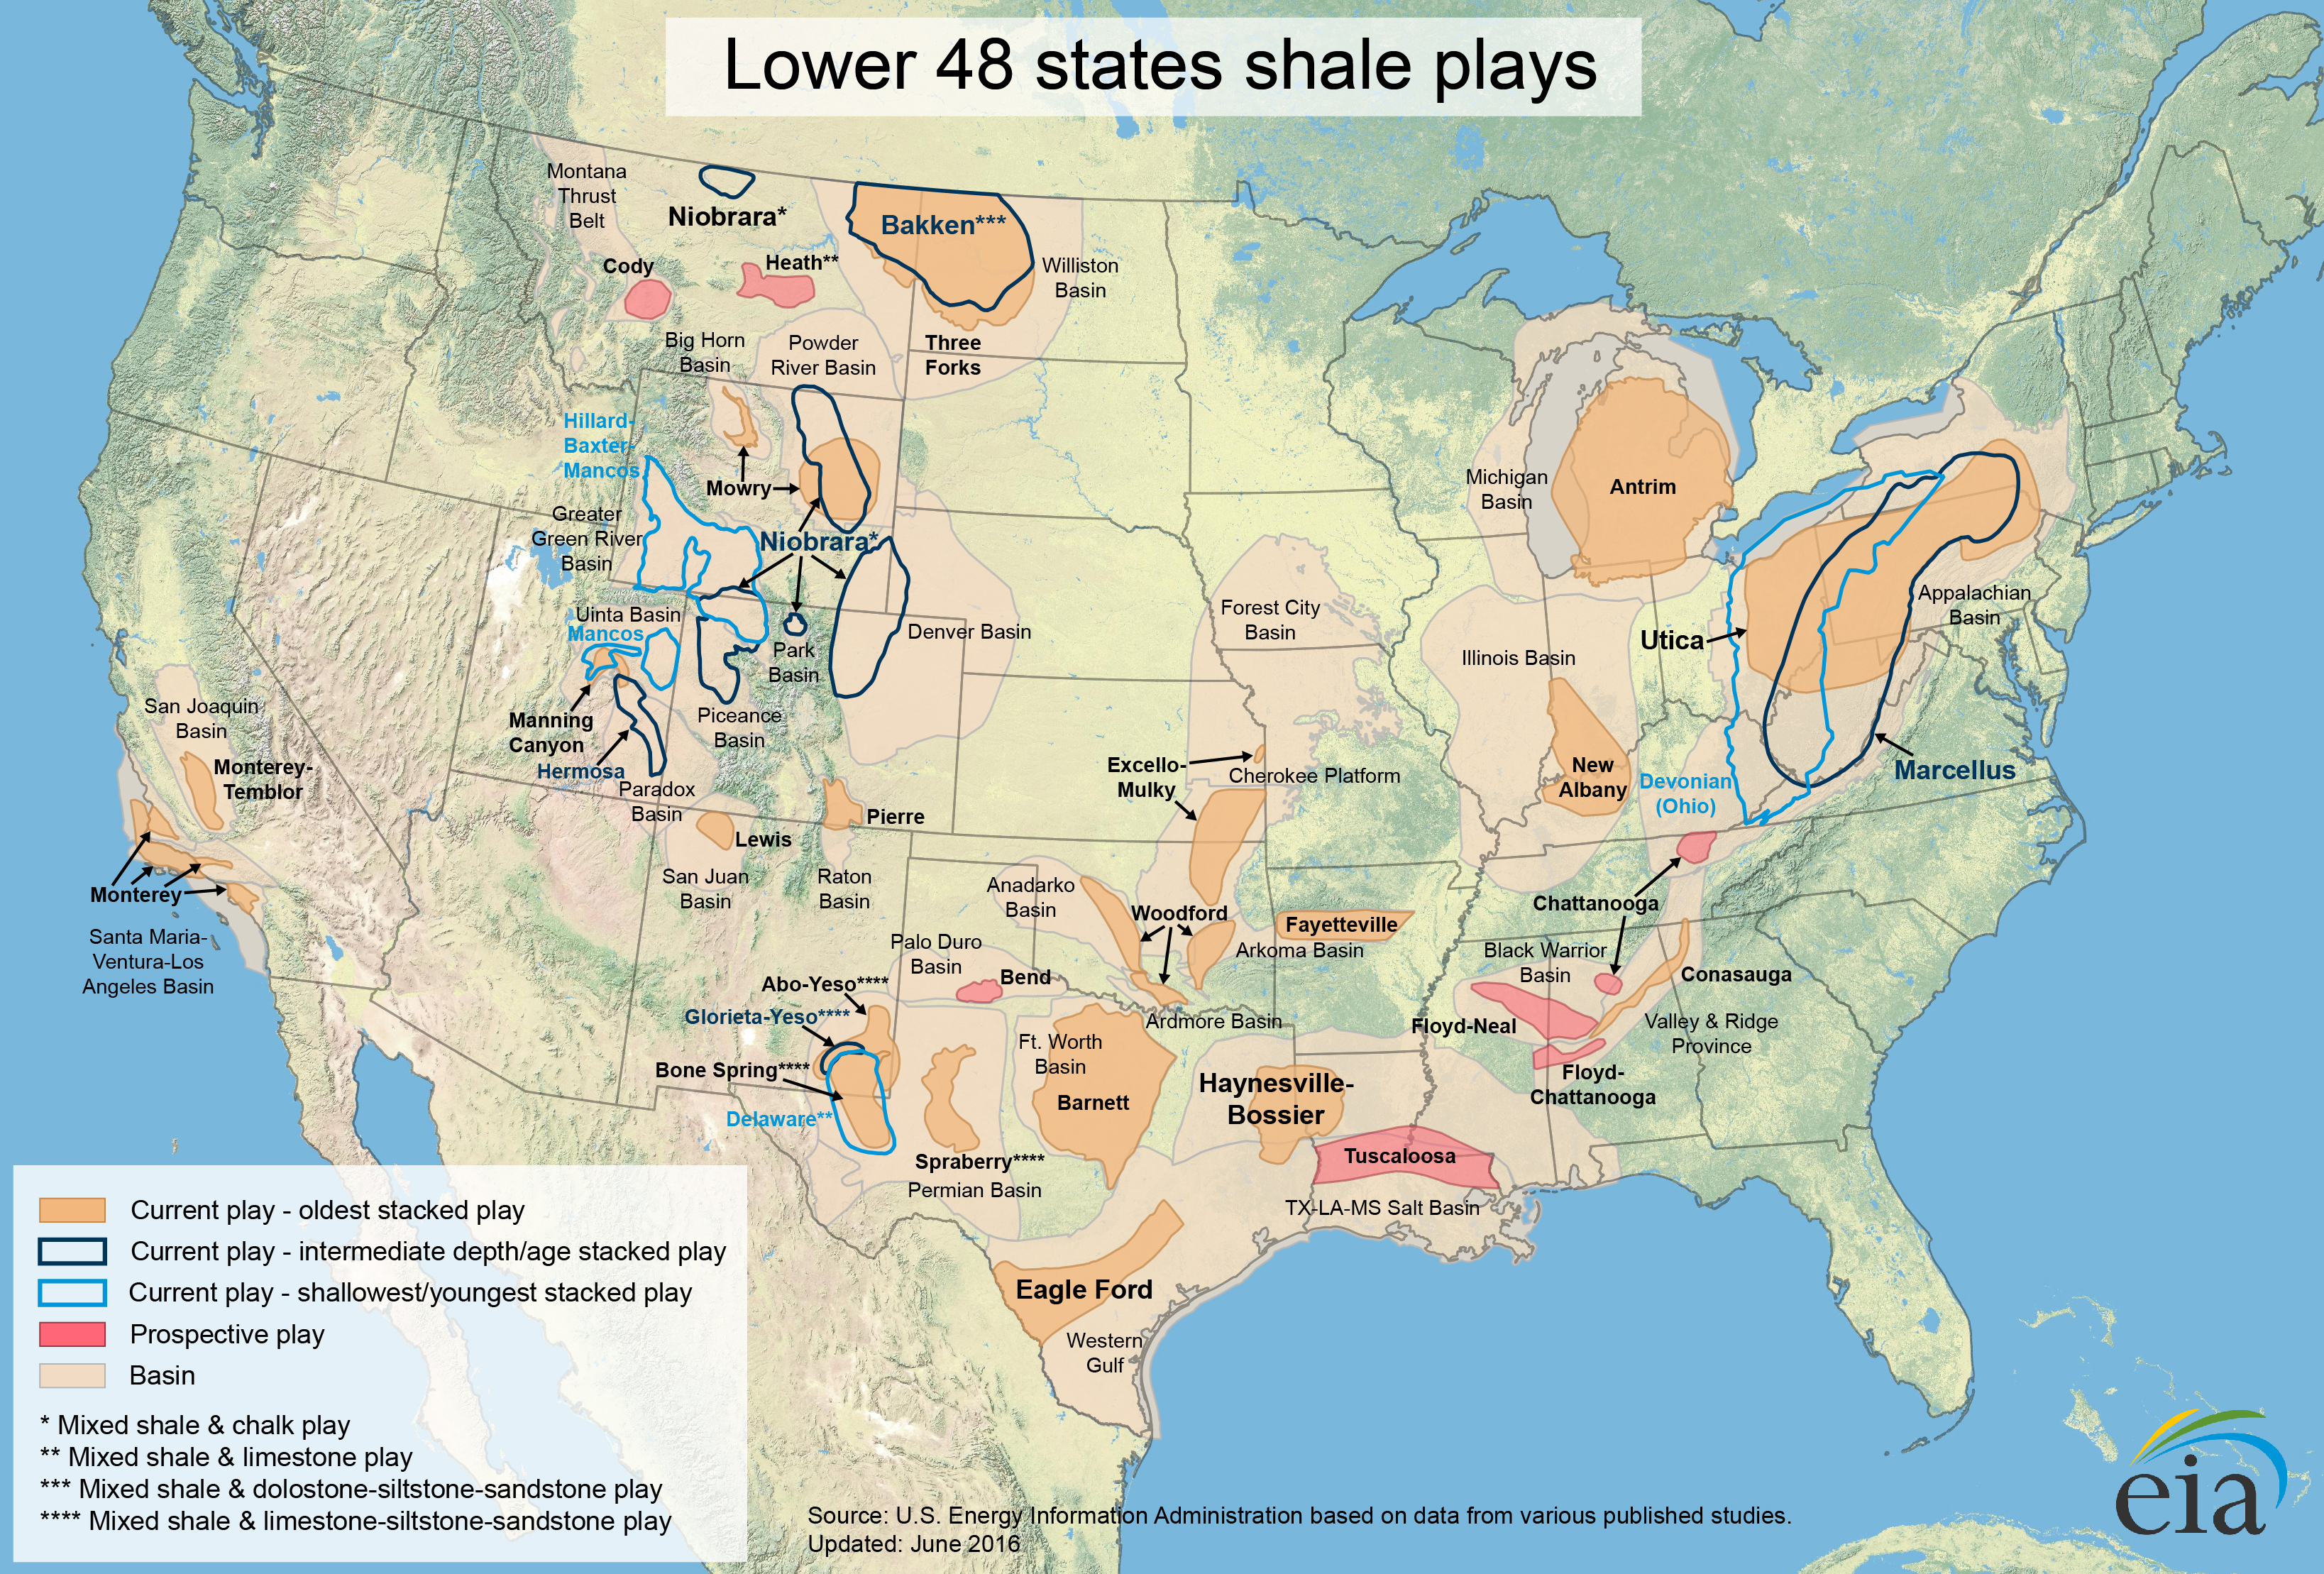
\includegraphics{https://www.eia.gov/maps/images/shale_gas_lower48.jpg}

\end{frame}

\begin{frame}{Fracking Well. Will see with oil well with associated gas}
\protect\hypertarget{fracking-well.-will-see-with-oil-well-with-associated-gas}{}

\includegraphics{https://fm.cnbc.com/applications/cnbc.com/resources/img/editorial/2012/06/12/47784444-Nat-gas-fracking-the-well.jpg}

\end{frame}

\begin{frame}{How do you move it within the US? Pipelines.}
\protect\hypertarget{how-do-you-move-it-within-the-us-pipelines.}{}

\includegraphics{https://upload.wikimedia.org/wikipedia/commons/4/47/Natural_gas_pipelines_map.png}

\end{frame}

\begin{frame}{What about those pipelines?}
\protect\hypertarget{what-about-those-pipelines}{}

\begin{itemize}
\tightlist
\item
  There are more intrastate pipelines than shown, plenty in TX and CA
  but also other states
\item
  Picture pipes ranging from a foot to three+ feet for trunk lines.
\item
  Compressor stations every 50-100 miles, \textasciitilde{}1,500 total
\item
  200 psi to 1,500 depending
\item
  They are privately owned

  \begin{itemize}
  \tightlist
  \item
    Open access, posted prices, is a thing.
  \item
    For intrastate, within, state PUC regulate
  \item
    For interstate, FERC regulates (You can find current Tariffs at
    \url{http://etariff.ferc.gov/TariffList.aspx})
  \end{itemize}
\end{itemize}

\end{frame}

\begin{frame}{Compressors}
\protect\hypertarget{compressors}{}

\includegraphics{https://stateimpact.npr.org/pennsylvania/files/2014/08/Compressor2-620x410.jpg}

\end{frame}

\begin{frame}{Compressor Station}
\protect\hypertarget{compressor-station}{}

\includegraphics{http://www.gdacoalition.org/GDAC_Images/CompressorStation1.JPG}

\end{frame}

\begin{frame}{Storage is important}
\protect\hypertarget{storage-is-important}{}

\includegraphics{https://www.eia.gov/todayinenergy/images/2015.11.16/chart3.png}

\end{frame}

\begin{frame}{Most Storage is just old gas wells}
\protect\hypertarget{most-storage-is-just-old-gas-wells}{}

\includegraphics{http://www.energyinfrastructure.org/~/media/energyinfrastructure/images/ng-storage/updated-2-18/typeofngstoragegraphic-218.png?la=en}

\end{frame}

\begin{frame}{Storage is very seasonal}
\protect\hypertarget{storage-is-very-seasonal}{}

There is a weekly report on storage by EIA
\url{http://www.eia.gov/dnav/ng/hist/nw2_epg0_swo_r48_bcfw.htm}

\begin{itemize}
\tightlist
\item
  Note the seasonality
\item
  Note the factor of 2+ changes over the term
\end{itemize}

\end{frame}

\begin{frame}{Hubs, where transactions are made}
\protect\hypertarget{hubs-where-transactions-are-made}{}

\includegraphics{MarketCenterHubsMap.gif}

\end{frame}

\begin{frame}{Part of Henry Hub LA}
\protect\hypertarget{part-of-henry-hub-la}{}

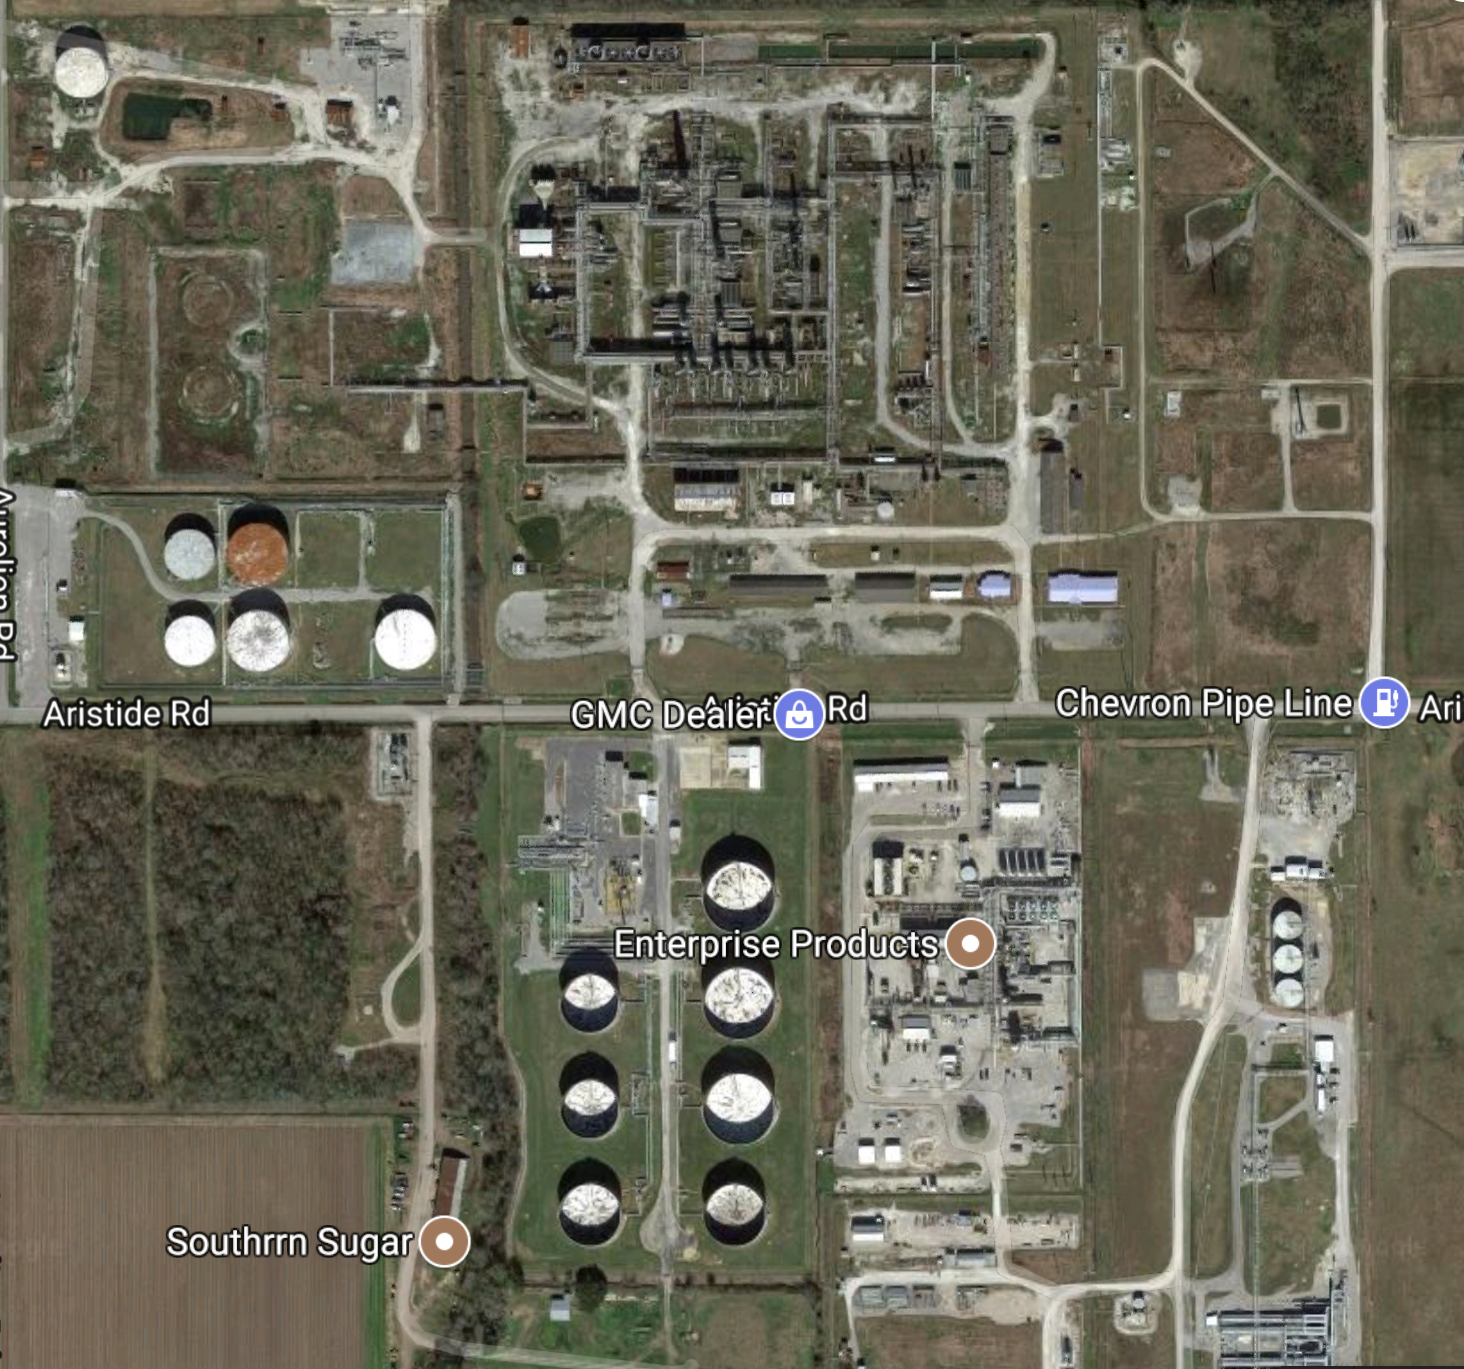
\includegraphics{PartHH.PNG}

\end{frame}

\begin{frame}{Getting to Prices}
\protect\hypertarget{getting-to-prices}{}

\begin{itemize}
\tightlist
\item
  You will see wellhead prices, but
\item
  Most references prices are at the hubs.

  \begin{itemize}
  \tightlist
  \item
    Henry Hub in LA is the most common reference hub for prices
  \item
    There are fairly firm relationships between other hubs and HH except
    when there is congestion.
  \item
    Changes in the usual difference are usually called basis blowout.
    Term is not specific to energy.
  \end{itemize}
\item
  Intercontinental Exchange for Gas Itself

  \begin{itemize}
  \tightlist
  \item
    \url{https://www.theice.com/products/OTC/Physical-Energy/Natural-Gas}
  \end{itemize}
\item
  FERC for transportation tariffs (Regulated)

  \begin{itemize}
  \tightlist
  \item
    \url{http://etariff.ferc.gov/TariffList.aspx}
  \item
    Some are fixed and some have a market rate component.
  \end{itemize}
\item
  EIA has easier access to prices
  \url{https://www.eia.gov/dnav/ng/hist/rngwhhdM.htm}
\end{itemize}

It is hard to talk about gas separate from transportation.

\end{frame}

\begin{frame}{Intro Deregulation in Natural Gas}
\protect\hypertarget{intro-deregulation-in-natural-gas}{}

\begin{itemize}
\tightlist
\item
  Transmission companies used to own the gas.

  \begin{itemize}
  \tightlist
  \item
    Buy on one end
  \item
    Sell on the other
  \end{itemize}
\item
  Natural Gas Policy Act of 1978 started the process \ldots{} but didn't
  work well
\item
  FERC 236 1985 simplified product definitions
\item
  FERC 636 in 1992 was were it really started.
\end{itemize}

\end{frame}

\begin{frame}{Key Points about Deregulation in General}
\protect\hypertarget{key-points-about-deregulation-in-general}{}

\begin{itemize}
\tightlist
\item
  The point is not to keep hands off and let the markets develop into
  whatever form they want.

  \begin{itemize}
  \tightlist
  \item
    There is a balance between minimizing transactions cost, which your
    book focuses on, and efficiency.
  \item
    Markets will tend to reduce transactions cost, merging etc, but that
    does not make for efficient allocation.
  \end{itemize}
\item
  The idea is to create market rules that balance allocative efficiency
  and transaction cost minimization.

  \begin{itemize}
  \tightlist
  \item
    Focus on all transactions being visible in some way. (Competition
    requires a good information environment)
  \item
    Focus on reducing market power (Why pipelines can't own the gas in
    them any more.)
  \item
    Open access (Law of one price)
  \item
    Put a price on everything

    \begin{itemize}
    \tightlist
    \item
      Storage
    \item
      Timing and reliability of transport access
    \item
      Unbundling of prices.
    \end{itemize}
  \end{itemize}
\end{itemize}

\end{frame}

\begin{frame}{Transactions Cost Economics}
\protect\hypertarget{transactions-cost-economics}{}

Goes back to Coase 1937 (Nobel). Williamson (Nobel also). Elinor Ostrom
(Nobel too).

This just in Hart and Holstrom (2016 Nobel)

Transactions are not cost free:

\begin{itemize}
\tightlist
\item
  Search and information cost (Coordination)
\item
  Bargaining (Defining what you want)
\item
  Enforcement (Getting people to do what they said)
\item
  Strategic behavior (Hold Up Problem) Transaction specific investments
\end{itemize}

Minimizing Transaction Cost often means vertically integrating:

\begin{itemize}
\tightlist
\item
  Merge with your suppliers or with who you supply.
\item
  Working with only one internal supplier may minimize current costs but
  may not provide incentives to reduce further.
\item
  Larger firms often mean more market power in terminal market.
\end{itemize}

\end{frame}

\begin{frame}{Intent of regulation is to get closer to perfect
competition}
\protect\hypertarget{intent-of-regulation-is-to-get-closer-to-perfect-competition}{}

\begin{itemize}
\tightlist
\item
  Information rich
\item
  Minimized market power
\item
  Information is contained in prices
\item
  There are a lot of prices
\item
  Complex trading floor operations to control cost and risk.
\end{itemize}

\end{frame}

\end{document}
